\section{Active Target Time Projection Chambers}\label{sec:attpc}

\subsection{A note on nuclear physics}

In this thesis we primarily concern ourselves with analysis methods that are agnostic to the physics in the system. One can argue that this is both a strength of the methodology and a weakness. As a consequence the discussion of the physical system will brief. For a more in-depth treatment of the physics  see \cite{Bradt2017}. 

With that in mind we turn to the central pursuits of nuclear physics: understanding the structure of the nucleus. Nuclides are described in terms of the number of protons, $Z$, and neutrons $N$ and their total mass number $A = Z +N$. They are further categorized by equal components; nuclides with an equal number of protons are called \textit{isotopes}, equal number of neutrons \textit{isotones} and with the same  mass \textit{isobars}. The first modern fully-formed theory of nuclear structure, the nuclear shell model, was focused around the observation that certain isotopes and isotones were much more stable than others. As it happened these stable nuclei were regularly spaced around certain numbers of constituent protons and neutrons. These numbers are called magic numbers and describe nuclides that are much more tightly bound than the next number, as a consequence they are very stable and exhibit long half-lives. These magic numbers are: $2 ,\, 8 ,\, 20 ,\, 28 ,\, 50 ,\, 82 ,\, 126$. Some nuclides are even doubly-magic, which is to say both $Z$ and $N$ are magic numbers. One area of active research is around the $N=28$ isotones. Predictions from the nuclear shell model indicates that these isotones should have an approximately spherical structure. This has been disproved experimentally as deformities appear when removing protons from the spherical nucleus ${}^{48}Ca$. Which brings us to ${}^{46}Ar$ which lies in a region between the spherical ${}^{48}Ca$ and the lighter isotones that are known to be deformed. The location of ${}^{46}Ar$ makes it an object of some academic interest, and served as the commissioning of the AT-TPC (Active Target Time Projection Chamber) at the NSCL. 

% The AT-TPC is a charged particle detector built at the NSCL designed to capture events in the energy range $0.3\mega \eV \per u$ to  $6\mega \eV \per u$

\begin{figure}
\centering
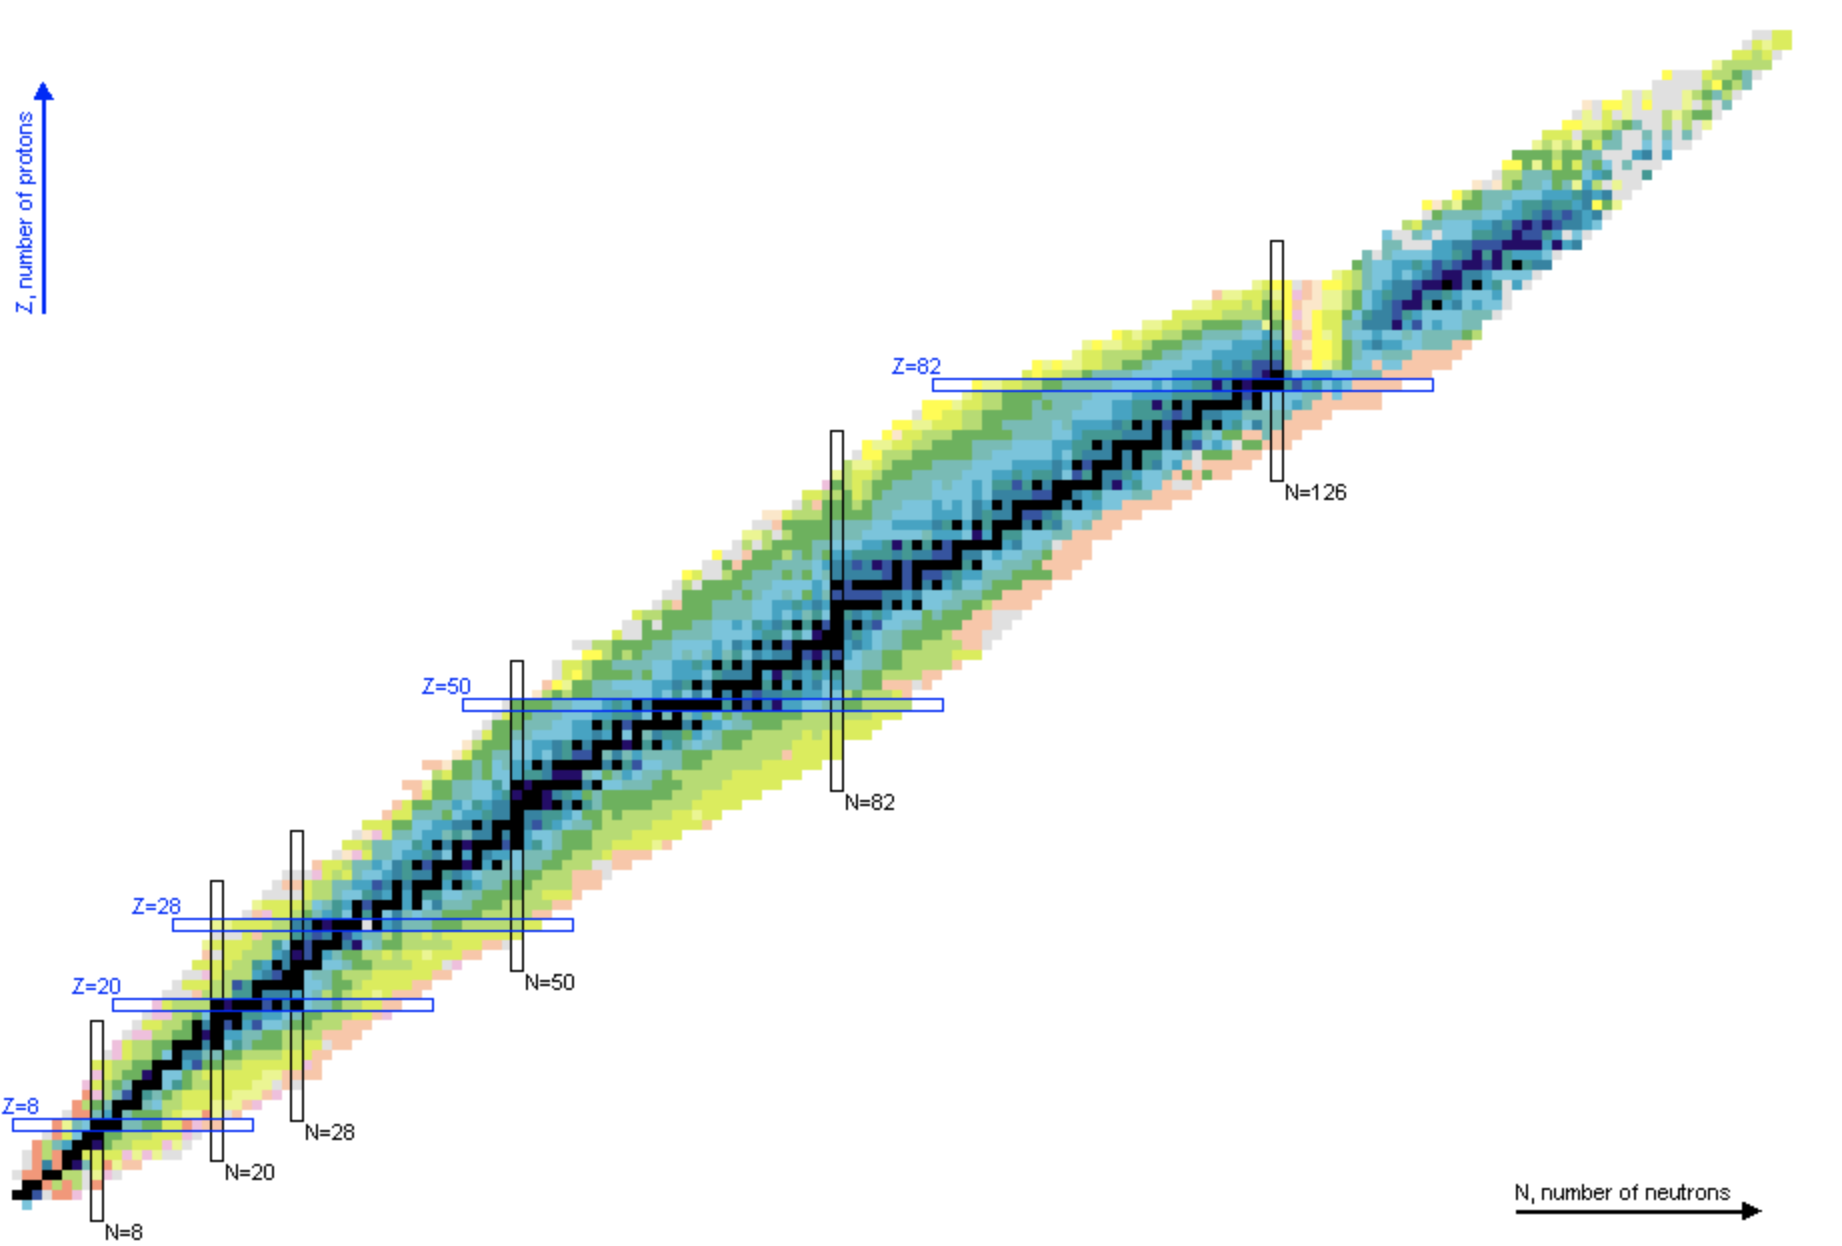
\includegraphics[width=\textwidth]{../plots/chart_nucleides}
\caption[Chart of the nuclides]{Chart of the known nuclides. The number of protons are given along the vertical axis, and neutrons along the horizontal. The color indicates the half-life of the nucleus with darker colors representing longer times. Lines of isotones and isotopes along the magic numbers are indicated by rectangles in the figure. Retrieved from \cite{Sonzogni2019}}
\end{figure}

\subsubsection{Isobaric analogues}

\subsection{AT-TPC details}


\begin{enumerate}
	\item Introduce the TPC and AT-TPC
	\item Introduce the objective and of the AT-TPC experiments
	\item Introduce and discuss the physics of the AT-TPC experiments 
	\item Discuss the need for ML in event categorization in the AT-TPC experiments 
\end{enumerate}